% ==================================================
%  Capítulo 4 — Análisis Exploratorio de Datos (EDA)
% ==================================================
\section{Análisis Exploratorio de Datos}\label{sec:eda}

Antes de entrenar cualquier modelo, se auditó el dataset consolidado con tres objetivos: verificar la integridad de los datos, caracterizar la distribución de las variables ópticas y extraer hallazgos que orientaran las decisiones de modelado. Esta auditoría fue determinante, ya que mostró que la métrica escalar de calidad ($R^2$) presenta un desbalance extremo hacia configuraciones de bajo desempeño. Este resultado motivó el re-encuadre metodológico del proyecto.

\subsection{Distribución de la Calidad de Enfoque}\label{subsec:estadisticas}

La Tabla~\ref{tab:stats_r2} y la Figura~\ref{fig:hist_r2} resumen la distribución del coeficiente $R^2$ en el dataset consolidado.

\begin{table}[H]
\centering
\small
\begin{tabular}{lc}
\toprule
\textbf{Métrica} & \textbf{Valor} \\
\midrule
Total de simulaciones            & 1{,}110 \\
$R^2$ mínimo / máximo            & 0.000 / 0.958 \\
$R^2$ promedio (mediana)         & 0.241 (0.160) \\
$R^2$ desviación estándar        & 0.239 \\
Simulaciones con $R^2 \geq 0.90$ & 4 \,(0.36\%) \\
Simulaciones con $R^2 \geq 0.85$ & 23 \,(2.07\%) \\
Simulaciones con $R^2 < 0.30$    & 753 \,(67.8\%) \\
\bottomrule
\end{tabular}
\caption{Estadísticas descriptivas del coeficiente de determinación $R^2$ en el dataset.}
\label{tab:stats_r2}
\end{table}

\begin{figure}[H]
    \centering
    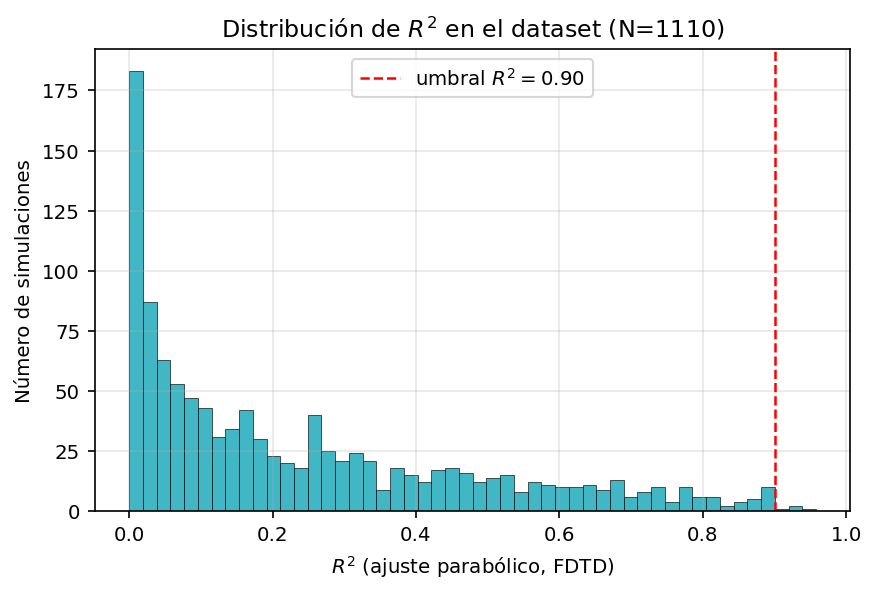
\includegraphics[width=0.62\textwidth]{Figuras/fig_hist_r2.png}
    \caption{Distribución de $R^2$ en el dataset ($N=1{,}110$). La gran mayoría de las
    configuraciones no produce enfoque; la región de interés ($R^2 \geq 0.90$, línea roja)
    es minúscula.}
    \label{fig:hist_r2}
\end{figure}

El valor promedio $R^2 \approx 0.24$ y la mediana $0.16$ muestran que la mayor parte de las geometrías simuladas no produce un enfoque satisfactorio bajo el criterio operativo adoptado. Este comportamiento es esperable dado que el diseño de experimentos no se concentró únicamente en geometrías tipo lente, sino que exploró un conjunto parametrizado de perfiles de ancho con respuestas ópticas diversas. Como resultado, el dataset contiene configuraciones que producen enfoque parcial, difracción, dispersión o patrones de intensidad sin una trayectoria focal claramente parabólica.

La presencia de abundantes ejemplos de bajo desempeño no es inútil, pues estas simulaciones aportan información sobre el mapeo geometría--respuesta óptica y ayudan al modelo a reconocer regiones no prometedoras del espacio explorado. Sin embargo, la escasez de ejemplos de alto $R^2$ limita severamente la posibilidad de aprender de forma global las condiciones geométricas que producen enfoque óptimo.

\subsection{Implicación para el Objetivo de Aprendizaje}\label{subsec:implicacion}

La observación central del EDA es que solo $4$ de $1{,}110$ simulaciones ($0.36\%$) alcanzan $R^2 \geq 0.90$. Tratar el problema como una clasificación binaria de calidad, por ejemplo enfocador ``frente a no enfocador'', implicaría un desbalance aproximado de ${\sim}1{:}277$. En ese escenario, un clasificador trivial que siempre predijera la clase mayoritaria obtendría una exactitud cercana al $99.6\%$ sin aprender una regla útil para identificar geometrías de alto desempeño.

Este desbalance no es solamente un inconveniente estadístico, sino una característica estructural del problema bajo el diseño de experimentos utilizado. Las configuraciones que satisfacen el criterio de alto $R^2$ ocupan una región muy pequeña del espacio parametrizado, por lo que técnicas como re-ponderación de clases o modificación del umbral de decisión pueden mejorar parcialmente el entrenamiento, pero no resuelven la falta de ejemplos suficientes alrededor de las regiones óptimas.

Por esta razón, el problema se reformuló como una regresión del campo óptico focal completo. En lugar de pedir al modelo que aprenda directamente un escalar escaso y altamente desbalanceado, se utiliza como objetivo una representación densa y continua de la respuesta electromagnética, los perfiles de amplitud y fase en el plano focal. Esta formulación permite que todas las simulaciones, incluidas aquellas que no alcanzan el umbral de enfoque, aporten información al aprendizaje del mapeo geometría--campo óptico.

El criterio $R^2 \geq 0.90$ no desaparece, pero cambia de papel. Deja de ser el objetivo directo de entrenamiento del modelo final y se conserva como una métrica operativa de evaluación y selección de candidatos. En particular, el $R^2$ calculado a partir de la respuesta predicha por el surrogate puede utilizarse para priorizar geometrías durante la búsqueda, pero el cumplimiento del criterio de éxito debe confirmarse mediante simulación FDTD directa.

\subsection{Caracterización del Campo Óptico Focal}\label{subsec:campo_focal}

Una vez identificado que el objetivo de aprendizaje no debía reducirse únicamente al escalar $R^2$, se caracterizaron las dos magnitudes principales que componen la representación densa utilizada por el modelo final: la amplitud $|E|(y)$ y la fase $\Phi(y)$ a lo largo del plano focal. La amplitud se normaliza respecto al pico de cada simulación, de modo que su valor máximo es $1$ por construcción y la señal codifica principalmente la forma transversal del lóbulo focal, no su magnitud absoluta. La fase se desenvuelve y se centra por su mediana, ya que un desfase global constante no modifica la estructura relativa del frente de onda. La Figura~\ref{fig:eda_campos} y la Tabla~\ref{tab:campo_stats} resumen el comportamiento de estas variables, contrastando configuraciones de alto $R^2$ ($R^2 \geq 0.85$) con configuraciones de bajo $R^2$ ($R^2 < 0.30$).

\begin{figure}[H]
\centering
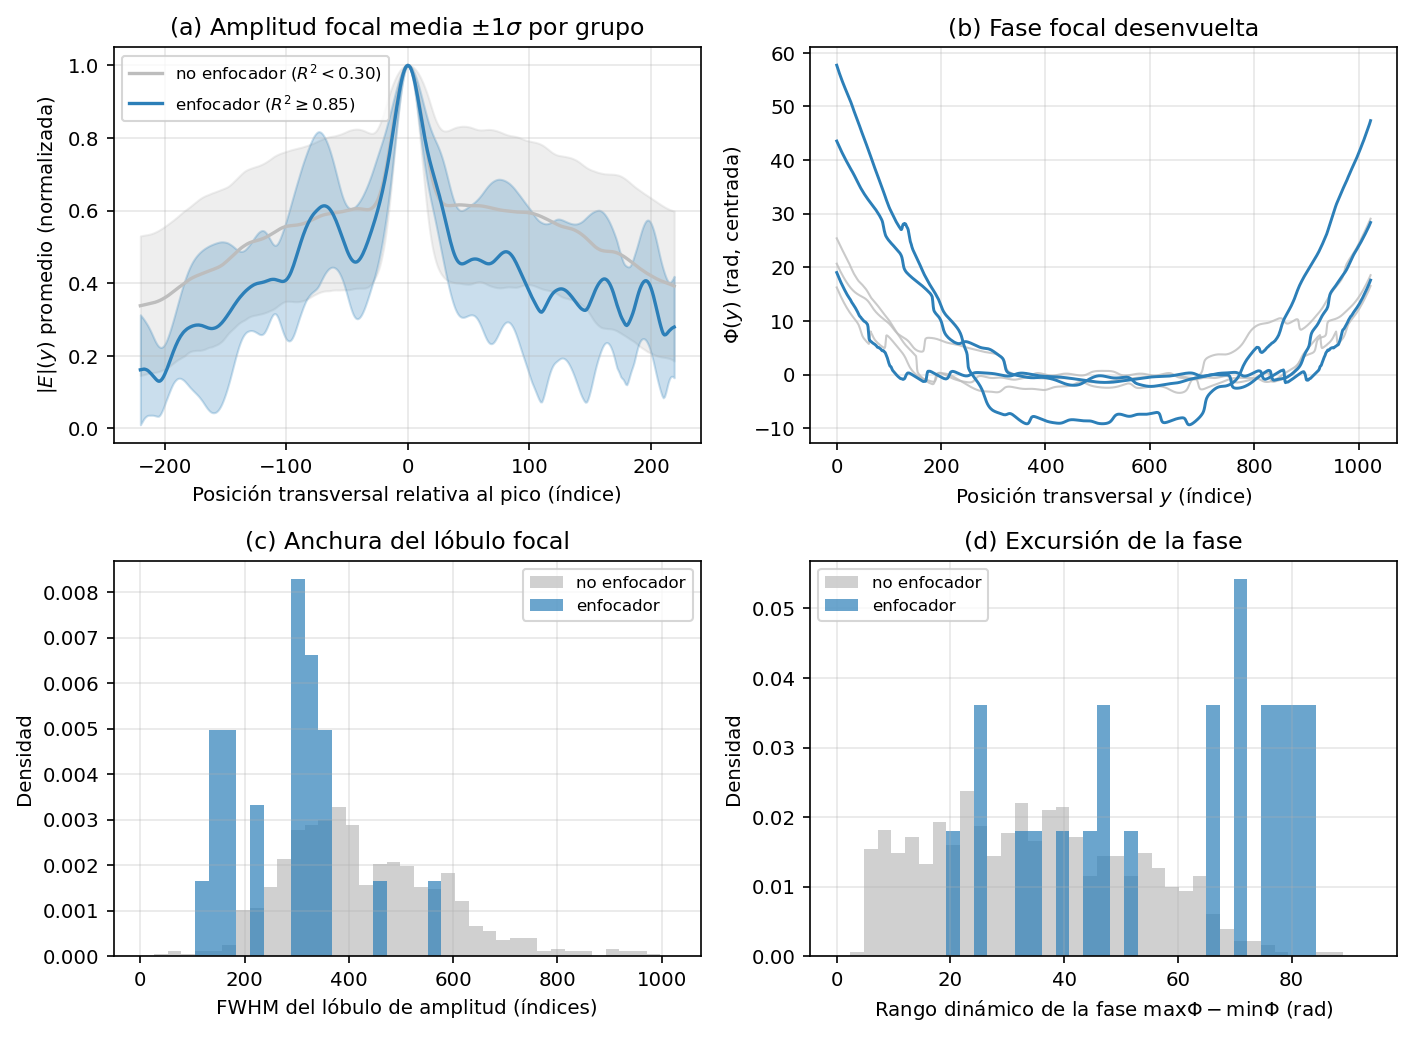
\includegraphics[width=\textwidth]{Figuras/fig_eda_campos.png}
\caption{Caracterización de los objetivos densos del modelo subrogado. (a)~Amplitud focal media alineada al pico por grupo: las configuraciones de alto $R^2$ muestran, en promedio, un lóbulo central más estrecho y localizado. (b)~Ejemplos representativos de fase focal desenvuelta: los casos de alto $R^2$ presentan mayor excursión y curvatura de fase. (c)~Distribución de la anchura a media altura (FWHM) del lóbulo de amplitud. (d)~Distribución del rango dinámico de la fase. Las distribuciones muestran desplazamientos sistemáticos entre grupos, aunque no una separación perfecta.}
\label{fig:eda_campos}
\end{figure}

\textbf{Amplitud.} El perfil de amplitud describe la distribución transversal de la luz en el plano focal. En las configuraciones de alto $R^2$, la amplitud tiende a concentrarse en un lóbulo central más estrecho: la anchura a media altura (FWHM) promedia $281$ índices frente a $426$ en las configuraciones de bajo $R^2$. De manera consistente, la fracción de energía contenida en el $10\%$ central alrededor del pico aumenta de $0.30$ a $0.41$ (Tabla~\ref{tab:campo_stats}; Figura~\ref{fig:eda_campos}a,c). Esta estructura sugiere que la amplitud focal contiene información discriminante sobre la calidad de enfoque. Además, al estar normalizada y acotada en $[0,1]$, constituye un objetivo relativamente bien condicionado para el modelo predictivo.

\textbf{Fase.} La fase transversal presenta un rango dinámico más amplio, del orden de decenas de radianes, con una media global de $36.4$~rad. Las configuraciones de alto $R^2$ exhiben una excursión de fase mayor que las configuraciones de bajo $R^2$: el rango dinámico promedio aumenta de $34.4$ a $58.6$~rad, y la desviación estándar de la fase pasa de $9.7$ a $16.5$~rad (Figura~\ref{fig:eda_campos}b,d). Este comportamiento es consistente con frentes de onda más fuertemente modulados, capaces de redistribuir la energía hacia la región focal. A diferencia de la amplitud, la fase conserva variaciones finas y mayor variabilidad entre simulaciones, por lo que representa el componente más exigente de la respuesta óptica a modelar.

\begin{table}[H]
\centering
\small
\begin{tabular}{lccc}
\toprule
\textbf{Descriptor} & \textbf{Global} & \textbf{Alto $R^2$} & \textbf{Bajo $R^2$} \\
& ($N=1{,}110$) & ($R^2\geq0.85$, $n=23$) & ($R^2<0.30$, $n=753$) \\
\midrule
\multicolumn{4}{l}{Amplitud $|E|(y)$} \\
\quad FWHM del lóbulo (índices) & 414 & 281 & 426 \\
\quad Energía en $10\%$ central & 0.31 & 0.41 & 0.30 \\
\midrule
\multicolumn{4}{l}{Fase $\Phi(y)$} \\
\quad Rango dinámico (rad) & 36.4 & 58.6 & 34.4 \\
\quad Desviación estándar (rad) & 10.2 & 16.5 & 9.7 \\
\bottomrule
\end{tabular}
\caption{Descriptores del campo óptico focal en el dataset, reportados de forma global y por grupos de calidad. Las configuraciones de alto $R^2$ tienden a presentar lóbulos de amplitud más concentrados y una modulación de fase más amplia.}
\label{tab:campo_stats}
\end{table}

En conjunto, estos resultados muestran que el campo focal contiene estructura útil para el aprendizaje: las configuraciones de alto y bajo $R^2$ no solo difieren en una métrica escalar, sino también en propiedades físicas observables de amplitud y fase. Esta evidencia respalda la decisión de utilizar una representación densa del campo óptico como objetivo del modelo subrogado. Al mismo tiempo, la variabilidad observada, especialmente en la fase, justifica el uso de un modelo con capacidad no lineal y una evaluación posterior cuidadosa de sus errores de predicción.

\subsection{Variabilidad del Plano Focal}\label{subsec:variabilidad}

El número de puntos transversales del campo focal (\texttt{ny}) varía entre simulaciones, con un rango aproximado de $[571,1023]$. Esta variabilidad se debe a que el tamaño del dominio FDTD se ajusta dinámicamente según la apertura total de cada metalente. Para construir una representación uniforme apta para el entrenamiento, todos los perfiles de amplitud y fase se re-muestrean por interpolación a una longitud fija de $1{,}024$ puntos (Sección~\ref{subsubsec:reencuadre}).

La elección de $1{,}024$ puntos permite homogeneizar las salidas sin reducir la resolución respecto al máximo observado de $1{,}023$ puntos transversales. De esta manera, cada simulación queda representada por vectores comparables de amplitud y fase, preservando la información espacial necesaria para el modelado multisalida.

\subsection{Integridad de los Datos}\label{subsec:anomalias}

La auditoría verificó la ausencia de valores \texttt{NaN} o \texttt{Inf} en los vectores de amplitud y fase de las simulaciones consolidadas. También se revisó que el plano focal identificado dinámicamente se encontrara dentro del dominio válido de cada simulación y que los perfiles extraídos tuvieran dimensiones compatibles con el proceso de re-muestreo. Con estas verificaciones, el conjunto resultante se consideró apto para las etapas posteriores de modelado sin requerir descartes adicionales.

\subsection{Hallazgos Principales}\label{subsec:hallazgos_eda}

\begin{enumerate}
\item \textbf{Región de alto desempeño escasa:} solo $0.36\%$ de las configuraciones alcanza $R^2 \geq 0.90$. Esta baja frecuencia vuelve poco adecuado tratar el problema final como una clasificación binaria de enfoque y motiva el uso de una representación más informativa de la respuesta óptica.

\item \textbf{Distribución dominada por bajos valores de $R^2$:} el valor promedio $R^2 \approx 0.24$ indica que la mayoría de las geometrías simuladas no satisface el criterio operativo de enfoque. Sin embargo, estas configuraciones siguen siendo útiles, ya que aportan información sobre regiones no prometedoras y sobre la variabilidad general del mapeo geometría--respuesta óptica.

\item \textbf{Campo focal con señal física relevante:} los perfiles de amplitud y fase muestran diferencias sistemáticas entre configuraciones de alto y bajo $R^2$. En particular, los casos de alto desempeño tienden a presentar lóbulos de amplitud más concentrados y una mayor excursión de fase. Esto respalda la decisión de utilizar el campo focal completo como objetivo del modelo subrogado.

\item \textbf{Fase como componente más exigente:} la fase desenvuelta presenta mayor rango dinámico y variabilidad que la amplitud, por lo que se anticipa como el componente más difícil de predecir. Esta observación orienta la evaluación posterior del modelo y la interpretación diferenciada de los errores en amplitud y fase.

\item \textbf{Necesidad de una estrategia de búsqueda controlada:} la combinación de alta dimensionalidad, familias parametrizadas de diseño y escasez de ejemplos de alto $R^2$ sugiere que el modelo subrogado será más útil como herramienta de priorización dentro de regiones exploradas que como evaluador global. Este hallazgo conecta el análisis exploratorio con la estrategia de optimización restringida descrita en la Sección~\ref{sec:optimizacion}.

\end{enumerate}
